\documentclass[12pt]{article}


\newcommand{\reporttitle}{Quantum Dots and Double Groups}
\newcommand{\reportauthor}{Michal Horanský}
\newcommand{\reporttype}{CMTH-Vvedensky-3}
\newcommand{\cid}{your college-id number}

%%%%%%%%%%%%%%%%%%%%%%%%%%%%%%%%%%%%%%%%%
% University Assignment Title Page 
% LaTeX Template
% Version 1.0 (27/12/12)
%
% This template has been downloaded from:
% http://www.LaTeXTemplates.com
%
% Original author:
% WikiBooks (http://en.wikibooks.org/wiki/LaTeX/Title_Creation)
%
% License:
% CC BY-NC-SA 3.0 (http://creativecommons.org/licenses/by-nc-sa/3.0/)
% 
% Instructions for using this template:
% This title page is capable of being compiled as is. This is not useful for 
% including it in another document. To do this, you have two options: 
%
% 1) Copy/paste everything between \begin{document} and \end{document} 
% starting at \begin{titlepage} and paste this into another LaTeX file where you 
% want your title page.
% OR
% 2) Remove everything outside the \begin{titlepage} and \end{titlepage} and 
% move this file to the same directory as the LaTeX file you wish to add it to. 
% Then add \input{./title_page_1.tex} to your LaTeX file where you want your
% title page.
%
%----------------------------------------------------------------------------------------
%	PACKAGES AND OTHER DOCUMENT CONFIGURATIONS
%----------------------------------------------------------------------------------------
\usepackage{ifxetex}
\usepackage{textpos}
%\usepackage{natbib}
%\usepackage{kpfonts}
\usepackage{amsfonts}
\usepackage[a4paper,hmargin=2.8cm,vmargin=2.0cm,includeheadfoot]{geometry}
\usepackage{ifxetex}
\usepackage{stackengine}
\usepackage{tabularx,longtable,multirow,subfigure,caption}%hangcaption
\usepackage{fncylab} %formatting of labels
\usepackage{fancyhdr}
\usepackage{color}
\usepackage[tight,ugly]{units}
\usepackage{url}
\usepackage{float}
\usepackage[english]{babel}
\usepackage{amsmath}
\usepackage{graphicx}
\usepackage[colorinlistoftodos]{todonotes}
\usepackage{dsfont}
\usepackage{epstopdf} % automatically replace .eps with .pdf in graphics
\usepackage{natbib}
%\usepackage{backref}
\usepackage{array}
\usepackage{latexsym}
\usepackage{etoolbox}

\usepackage{enumerate} % for numbering with [a)] format 

\usepackage{physics}
\usepackage{siunitx}

\usepackage{multirow}

\ifxetex
\usepackage{fontspec}
\setmainfont[Scale=.8]{OpenDyslexic-Regular}
\else
\usepackage[pdftex,hypertexnames=false,colorlinks]{hyperref} % provide links in pdf
\hypersetup{pdftitle={},
  pdfsubject={}, 
  pdfauthor={\reportauthor},
  pdfkeywords={}, 
  pdfstartview=FitH,
  pdfpagemode={UseOutlines},% None, FullScreen, UseOutlines
  bookmarksnumbered=true, bookmarksopen=true, colorlinks,
    citecolor=black,%
    filecolor=black,%
    linkcolor=black,%
    urlcolor=black}
\usepackage[all]{hypcap}
\fi

\usepackage{tcolorbox}

% various theorems
\usepackage{ntheorem}
\theoremstyle{break}
\newtheorem{lemma}{Lemma}
\newtheorem{theorem}{Theorem}
\newtheorem{remark}{Remark}
\newtheorem{definition}{Definition}
\newtheorem{proof}{Proof}

% example-environment
\newenvironment{example}[1][]
{ 
\vspace{4mm}
\noindent\makebox[\linewidth]{\rule{\hsize}{1.5pt}}
\textbf{Example #1}\\
}
{ 
\noindent\newline\makebox[\linewidth]{\rule{\hsize}{1.0pt}}
}



%\renewcommand{\rmdefault}{pplx} % Palatino
% \renewcommand{\rmdefault}{put} % Utopia

\ifxetex
\else
\renewcommand*{\rmdefault}{bch} % Charter
\renewcommand*{\ttdefault}{cmtt} % Computer Modern Typewriter
%\renewcommand*{\rmdefault}{phv} % Helvetica
%\renewcommand*{\rmdefault}{iwona} % Avant Garde
\fi

\setlength{\parindent}{0em}  % indentation of paragraph

\setlength{\headheight}{14.5pt}
\pagestyle{fancy}
\fancyfoot[ER,OL]{\thepage}%Page no. in the left on
                                %odd pages and on right on even pages
\fancyfoot[OC,EC]{\sffamily }
\renewcommand{\headrulewidth}{0.1pt}
\renewcommand{\footrulewidth}{0.1pt}
\captionsetup{margin=10pt,font=small,labelfont=bf}


%--- chapter heading

\def\@makechapterhead#1{%
  \vspace*{10\p@}%
  {\parindent \z@ \raggedright %\sffamily
        %{\Large \MakeUppercase{\@chapapp} \space \thechapter}
        %\\
        %\hrulefill
        %\par\nobreak
        %\vskip 10\p@
    \interlinepenalty\@M
    \Huge \bfseries 
    \thechapter \space\space #1\par\nobreak
    \vskip 30\p@
  }}

%---chapter heading for \chapter*  
\def\@makeschapterhead#1{%
  \vspace*{10\p@}%
  {\parindent \z@ \raggedright
    \sffamily
    \interlinepenalty\@M
    \Huge \bfseries  
    #1\par\nobreak
    \vskip 30\p@
  }}
  



% %%%%%%%%%%%%% boxit
\def\Beginboxit
   {\par
    \vbox\bgroup
	   \hrule
	   \hbox\bgroup
		  \vrule \kern1.2pt %
		  \vbox\bgroup\kern1.2pt
   }

\def\Endboxit{%
			      \kern1.2pt
		       \egroup
		  \kern1.2pt\vrule
		\egroup
	   \hrule
	 \egroup
   }	

\newenvironment{boxit}{\Beginboxit}{\Endboxit}
\newenvironment{boxit*}{\Beginboxit\hbox to\hsize{}}{\Endboxit}



\allowdisplaybreaks

\makeatletter
\newcounter{elimination@steps}
\newcolumntype{R}[1]{>{\raggedleft\arraybackslash$}p{#1}<{$}}
\def\elimination@num@rights{}
\def\elimination@num@variables{}
\def\elimination@col@width{}
\newenvironment{elimination}[4][0]
{
    \setcounter{elimination@steps}{0}
    \def\elimination@num@rights{#1}
    \def\elimination@num@variables{#2}
    \def\elimination@col@width{#3}
    \renewcommand{\arraystretch}{#4}
    \start@align\@ne\st@rredtrue\m@ne
}
{
    \endalign
    \ignorespacesafterend
}
\newcommand{\eliminationstep}[2]
{
    \ifnum\value{elimination@steps}>0\leadsto\quad\fi
    \left[
        \ifnum\elimination@num@rights>0
            \begin{array}
            {@{}*{\elimination@num@variables}{R{\elimination@col@width}}
            |@{}*{\elimination@num@rights}{R{\elimination@col@width}}}
        \else
            \begin{array}
            {@{}*{\elimination@num@variables}{R{\elimination@col@width}}}
        \fi
            #1
        \end{array}
    \right]
    & 
    \begin{array}{l}
        #2
    \end{array}
    &%                                    moved second & here
    \addtocounter{elimination@steps}{1}
}
\makeatother

%% Fast macro for column vectors
\makeatletter  
\def\colvec#1{\expandafter\colvec@i#1,,,,,,,,,\@nil}
\def\colvec@i#1,#2,#3,#4,#5,#6,#7,#8,#9\@nil{% 
  \ifx$#2$ \begin{bmatrix}#1\end{bmatrix} \else
    \ifx$#3$ \begin{bmatrix}#1\\#2\end{bmatrix} \else
      \ifx$#4$ \begin{bmatrix}#1\\#2\\#3\end{bmatrix}\else
        \ifx$#5$ \begin{bmatrix}#1\\#2\\#3\\#4\end{bmatrix}\else
          \ifx$#6$ \begin{bmatrix}#1\\#2\\#3\\#4\\#5\end{bmatrix}\else
            \ifx$#7$ \begin{bmatrix}#1\\#2\\#3\\#4\\#5\\#6\end{bmatrix}\else
              \ifx$#8$ \begin{bmatrix}#1\\#2\\#3\\#4\\#5\\#6\\#7\end{bmatrix}\else
                 \PackageError{Column Vector}{The vector you tried to write is too big, use bmatrix instead}{Try using the bmatrix environment}
              \fi
            \fi
          \fi
        \fi
      \fi
    \fi
  \fi 
}  
\makeatother

\robustify{\colvec}

%%% Local Variables: 
%%% mode: latex
%%% TeX-master: "notes"
%%% End: 

\usepackage{caption}
% correct bad hyphenation here
\hyphenation{op-tical net-works semi-conduc-tor}

\begin{document}

%\title{Double Groups and Quantum Dots - Literature Review}%
%\author{Michal Horansky}

%\markboth{M. HORANSKY}%
%{Horansky \MakeLowercase{\textit{et al.}}:}

%\maketitle

% Last modification: 2016-09-29 (Marc Deisenroth)
\begin{titlepage}

\newcommand{\HRule}{\rule{\linewidth}{0.5mm}} % Defines a new command for the horizontal lines, change thickness here


%----------------------------------------------------------------------------------------
%	LOGO SECTION
%----------------------------------------------------------------------------------------


\includegraphics[width = 4cm]{./figures/imperial}\\[0.5cm] 

\begin{center} % Center remainder of the page

%----------------------------------------------------------------------------------------
%	HEADING SECTIONS
%----------------------------------------------------------------------------------------
\textsc{\LARGE \reporttype}\\[1.5cm] 
\textsc{\Large Imperial College London}\\[0.5cm] 
\textsc{\large Department of Physics}\\[0.5cm] 
%----------------------------------------------------------------------------------------
%	TITLE SECTION
%----------------------------------------------------------------------------------------

\HRule \\[0.4cm]
{ \huge \bfseries \reporttitle}\\ % Title of your document
\HRule \\[1.5cm]
\end{center}
%----------------------------------------------------------------------------------------
%	AUTHOR SECTION
%----------------------------------------------------------------------------------------

%\begin{minipage}{0.4\hsize}
\begin{flushleft} \large
\textit{Author CID:}\\
\cid\\
\hfill\\
\textit{Supervisor:}\\
Prof Dimitri D. Vvedensky\\
\hfill\\
\textit{Assessor:}\\
Dr Paul Tangney\\
\hfill\\
\textit{Word count:}\\
9,850
\end{flushleft}
\vspace{2cm}
\makeatletter
Date: \@date 

\vfill % Fill the rest of the page with whitespace



\makeatother


\end{titlepage}




\begin{abstract}

In this project, we investigate the photonic properties of quantum dots employing an approach analogous to standard procedures in studies of the topic. Experimental data from polarisation resolved photoluminiscence spectroscopy are investigated using the theory of exciton complexes and group theory. The major features of the spectral diagrams can be labelled by exciton state transitions immediately by considering the properties of states of these exciton complexes. These major features also exhibit splitting caused by fine-structure spin interactions. This splitting is modelled using double groups, and agreement with polarisation and intensity of each resolvable peak is assessed. Predictions for dark and unresolved peaks are stated. Possible symmetry elevations in the quantum dot are discussed with consideration for their effects on the observed spectra.

\end{abstract}


\section{Introduction}
Quantum dots (QDs) have been the subject of keen interest and study by the scientific community in the last decades for their wide applications in quantum information (\cite{quantum_information1}), photonics (\cite{photonics1}, \cite{photonics2}), medicine (\cite{medicine1}, \cite{medicine2}) and many others (\cite{other_applications}). Many of these applications are viable due to the unique electronic properties of QDs that allow us to construct within it atom-like electron states \cite{atomlike} with tunable energy levels \cite{tunable} which depend on the specific manufacturing parameters. However, there are still challenges in characterising the small-scale structural properties of grown QDs, such as unintentional symmetry breaking \cite{karlsson}. In the project, we will inspect these structural properties using the tools of spectroscopy and the mathematical toolset of group theory.

Quantum dots are semiconductor nanocrystals \cite{other_applications}, which enjoy programmable charge states of electrons and electron holes (together dubbed exciton complexes) \cite{charge_state}. The most direct way to experimentally investigate the energy states of electrons and electron holes in QDs is photoluminiscence spectroscopy, a technique used in \cite{karlsson}. The QDs are first non-resonantly excited by a laser and then they spontaneously emit photons as a result of state transitions of exciton complexes. The spectrum of these emissions is given by the allowed state transitions. Hence, if each exciton complex state had a single associated energy, we could use standard arguments to determine which state transitions are allowed and with these transitions we would label each peak on the spectral diagram. However, there are complications that require further analysis to successfully label the spectral features of QD photoluminiscence. First, the properties of the crystallic structure of QDs may allow electron holes with different characteristics, which have to be labelled separately and which contribute to more allowed state transitions \cite{karlsson2}. Second, the exciton complexes enjoy spin-orbit coupling, which results in fine-structure splitting of energy levels \cite{fine-structure} (see Fig. \ref{fig:decay_diagrams}). Techniques analogous to that of Karlsson \textit{et al} in \cite{karlsson} are employed to properly analyse the first complication; similarly, their group theory approach will be used in our case as well to investigate the fine-structure effects.

\begin{figure}
\begin{center}
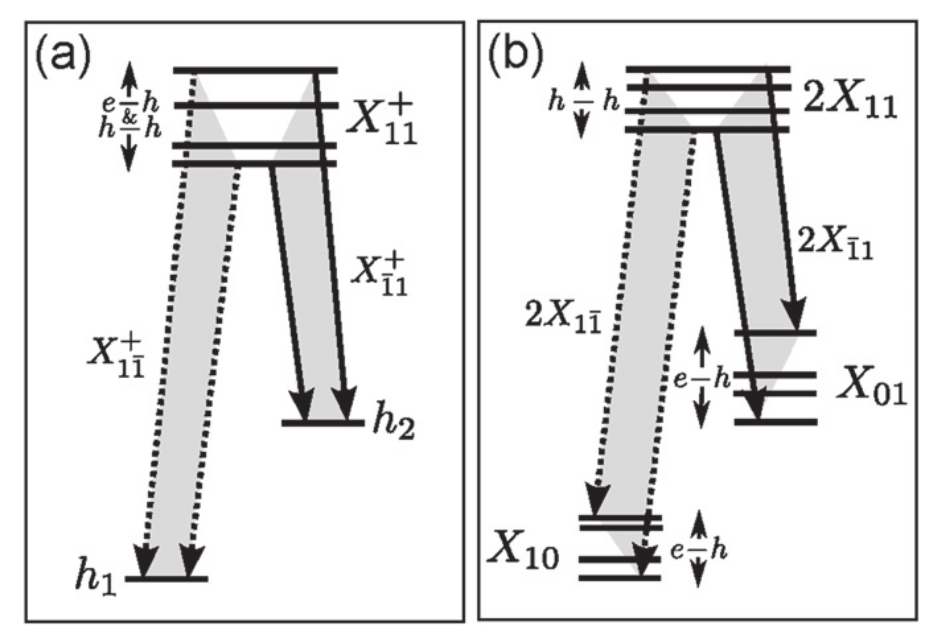
\includegraphics[scale=0.3]{figures/example_decay_diagrams}
\end{center}
\caption{Example of simple decay diagrams for a trion and a biexciton respectively. The subscripts indicate the occupancy of heavy-like and light-like holes in each exciton complex, and the superscript indicates the net charge. We see that clusters of energy levels are labelled by exciton complexes, but these clusters consist of multiple energy levels separated due to fine-structure splittings. Figure courtesy of Karlsson \textit{et al}, \cite{karlsson}.}
\label{fig:decay_diagrams}
\end{figure}
	
The utility of group theory in the study of spin-orbit interaction stems from the fact that degeneracies of energy levels are associated with symmetries. By considering the point group associated with the symmetry of the QD crystallic structure and then finding its double group, we can immediately write down the amount of different energy levels of a given exciton complex, their degeneracies, and even the allowed transitions with their polarisation for each energy level \cite[Ch. 19]{dresselhaus}. These values do not necessarily have to agree with the measured spectra, which is the crux of our uncertainty about the true QD structural symmetry -- this effect is called \textit{symmetry elevation}, and has been studied in \cite{karlsson2}. Hence, we need to consider potential symmetry breakings of the growth-mode crystallic structure for different transitions and assess the agreement of group theory predictions with the measured spectra.

\section{Background Material}

The main research paper our project will draw from shall be \cite{karlsson}, as it directly studies the structural properties of pyramidal GaAs quantum dots with (presumed) $C_{3v}$ symmetry that have been studied by Hartmann \textit{et al} in \cite{pyramidal_qds}, employing in order all the techniques that we wish to implement for the study of our system.

\subsection{Exciton analysis}
First, the specifics of the Brillouin zones of the QD crystallic structure can allow multiple characters of involved elementary particles -- for example, zincblende quantum wells have two different effective masses for holes in the valence band, referred to as heavy-like and light-like holes, which are labelled by separate quantum numbers and are associated with different polarisations \cite{karlsson2}. As noted by Karlsson \textit{et al} in \cite{karlsson}, the photoluminiscence intensity in the different hole regimes scales differently with crystal temperature, which Karlsson \textit{et al} conjectures to be the result of acoustic phonon relaxation bottleneck, an effect predicted by Bockelmann and Bastard \cite{bastard} and observed by Brunner \textit{et al} \cite{brunner}. This allows us to identify the characters of holes in transitions associated with peaks in the spectrum based on how the intensity of the peak changes with temperature, combined with the change in polarisation of emitted photons (see Fig. \ref{fig:temperature}). Then, a range of methods can be used to label certain peaks with a corresponding exciton complex decay transition.

\begin{figure}
\begin{center}
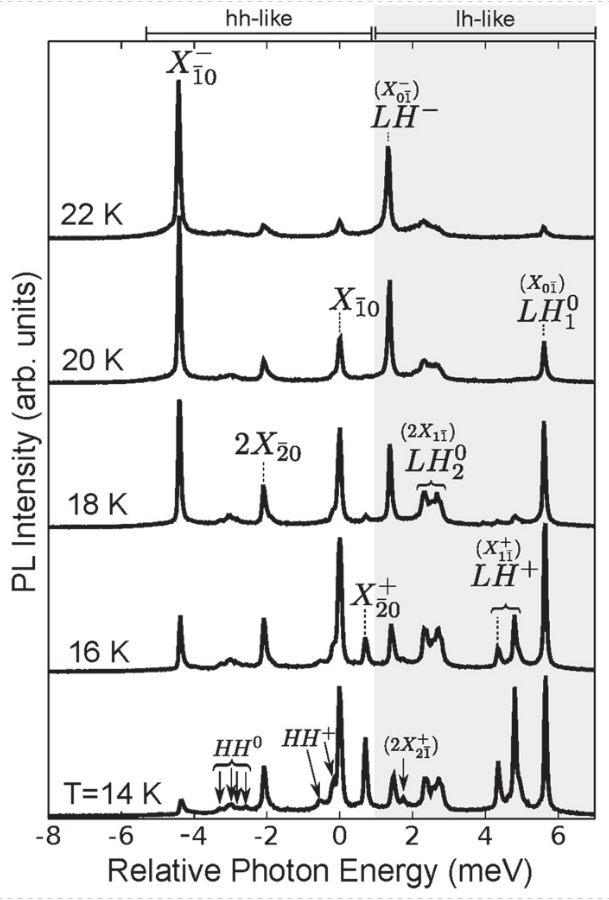
\includegraphics[scale=0.6]{figures/temperature_dependence}
\end{center}
\caption{Illustration of differing temperature dependence for various exciton complex-associated optical transitions for a pyramidal QD. This effect can be used to identify the major spectral features for other QDs as well. Figure courtesy of Karlsson \textit{et al}, \cite{karlsson}.}
\label{fig:temperature}
\end{figure}

\subsection{Coulomb interaction analysis}
Karlsson \textit{et al} employ the analysis of Coulomb interaction of exciton complexes to label the remaining peaks in the spectrum. More specifically, they use first-order approximations of Coulomb interactions between a system of electrons and holes in a quantum well to create a system of linear equations which relates the energies of decay transitions between several exciton complexes. By considering this approximation also for decays that have already been labelled by direct exciton analysis, Karlsson \textit{et al} are able to draw conclusions about the ordering of magnitudes of these decays, as well as the magnitudes of their variations on the spectral diagram, which is used both to finalise the labelling of all spectral features, as well as predicting the scaling of each peak with parameters such as the depth of the quantum well and its dimensions.

These techniques can be used analogously on quantum dots with other structural properties, making them useful for our project, although the necessary experimental data has to be obtained, such as the dynamics of charging and recombination of QDs under photoexcitation (for pyramidal QDs done by Baier \textit{et al} in \cite{pyramid_dynamics} using temporal photon-correlation spectroscopy) and the temperature dependences of specific decay transitions (for pyramidal QDs done e.g. by Karlsson \textit{et al} in \cite{pyramid_temperature}).

\subsection{Symmetry analysis}

We have thus far summarised the methods of labelling spectral features of quantum dot photoluminiscence. These techniques provide insight into the inner mechanisms of quantum dot spectroscopy, however, the body of original work in our project will consist mainly of the analysis of \textit{symmetries} of crystals that should explain the experimental measurements obtained by other researchers. For this, we will use the invaluable toolset provided by group theory, particularly the concept of double groups.

\begin{figure}
\begin{center}
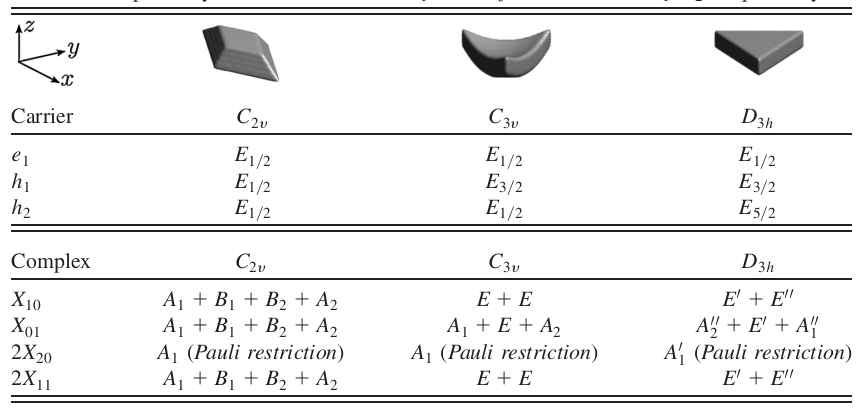
\includegraphics[scale=0.45]{figures/quantum_dot_symmetries}
\end{center}
\caption{Examples of symmetries for QD states for individual carriers and their exciton complexes. To obtain the spin-orbit coupling splitting levels, we first need to label the individual carriers by irreducible representations on the basis of simple symmetry arguments as per the work of Dupertuis \textit{et al} \cite{dupertuis}, and then consider the reducible representations of single excitons using the approach described by Dresselhaus \cite[Ch. 19]{dresselhaus}. Labelling multi-electron exciton complexes usually requires additional consideration of the Pauli exclusion principle, which forces certain symmetries. Figure courtesy of Dupertuis \textit{et al}, \cite{dupertuis}.}
\label{fig:symmetries}
\end{figure}

Double groups are groups built upon classic point groups that model symmetries of crystallic structures. When a half-integer spin particle, such as an electron, is introduced, states with half-integer angular momentum become allowed, expanding the number of symmetry operators. More specifically, the wavefunctions of eigenstates are now no longer periodic under rotation with a period of $2\pi$, but rather with a period of $4\pi$, as a $2\pi$ rotation requires the change of sign of a half-integer angular momentum wavefunction--this $4\pi$-periodicity has been confirmed experimentally by Werner \textit{et al} in \cite{fermion_periodicity}. Therefore, the identity element $E$ can now be understood as a rotation by $4\pi$, and rotation by $2\pi$ becomes a new symetry operation commonly denoted $\mathcal{R}, \mathcal{R}^2=E$. Consequently, for each symmetry operator $g$ a new symmetry operator is introduced, equal to $\mathcal{R}g$, doubling the group order (hence the name double group). A complex but trivial technique as shown in \cite{heine} is then used to find the new conjugacy classes and irreducible representations, the amounts of which are usually less than double of that for the original point group. One of these new representations, the representation of the spin function ($E_{1/2}$ in Mulliken notation), is unique since pure spin states transform as this representation. Therefore, if we consider the eigenfunctions of the new Hamiltonian as linear combinations of pure spin-up and pure spin-down Bloch eigenfunctions of the original crystallic structure, we see that they have to transform as both the representation of the specific Bloch eigenfunction and the dipole representation. Therefore the representations of the new eigenstates will usually be reducible, and can be decomposed from $\Gamma_i\otimes E_{1/2}$ into several irreducible representations of the double group, each labelling an energy level. Therefore, this directly gives us the energy levels of the fine-structure splitting and their degeneracies (see Fig. \ref{fig:symmetries}).
%the spin-orbit interaction term of the Hamiltonian%

The variance in polarisation of the emitted photons, which was used in classifying heavy-like and light-like electron holes, is also invaluable for assessing the predictions of group-theoretical analysis of symmetry, since it also includes information about polarisation associated with energy levels that emerge from fine-structure splitting. This is a simple consequence of the fact that these energy levels are labelled by irreducible representations of the point group of the quantum dot symmetries, such that all the eigenstates associated with a specific energy level transform as its irreducible representation \cite[Ch. 5]{dresselhaus}. Karlsson \textit{et al} employ the dipole approximation to consider how differently polarised photons transform according to different irreducible representations (the basis functions of irreducible representations can be found in standard tables, such as \cite{altmann}), which allows them to predict the polarisation of all allowed transitions.

\subsection{Symmetry elevation}
The techniques outlined above were employed by Karlsson \textit{et al} to study the structural symmetries of pyramidal QDs which are expected to exhibit $C_{3v}$ symmetry. However, the predicted energy splittings and allowed transitions did not agree with the measured spectral peaks for all exciton complexes. To explain this, Karlsson \textit{et al} conjectured that for certain complexes, the symmetry elevates to higher-symmetry point groups. For example, for the exciton $X_{10}$, symmetry elevation from $C_{3v}$ to $D_{3h}$ would forbid one predicted decay mode, which results in perfect agreement with the measured spectrum (one specific state of $X_{10}$ which is optically active in $C_{3v}$ symmetry becomes a dark state in $D_{3h}$ symmetry). Biexcitons $2X_{20}$ and $2X_{11}$ are also conjectured to experience symmetry elevation, and sensitive transitions whose presence in the spectrum probes the predicted symmetry are identified for other exciton complexes \cite{karlsson}. This outlines a very versatile toolset, which can be used to identify symmetry elevations for any exciton complex in a QD with any specific crystallic point group symmetry, as we will do in this project. This will illuminate the structural-symmetric properties of our studied QD system and how they vary in different states.

\section{Summary}
We have outlined our goal to probe the symmetry properties of a provided quantum dot structure using group theory approach to create a model that matches the measured polarisation-resolved photoluminiscence spectrum and predicts symmetry elevations for respective exciton states. An array of experiment-based arguments will be made to first label the photoluminiscence spectral peaks as decay modes of exciton complexes, and then the measured fine-structure energy splittings will be used as a basis for arguments about the symmetries of the respective quantum states, using the language of double groups. Our desired outcome for this project is a clear and concise point-group labelling of the first exciton complex states and the evaluation of the agreement between our predictions and the measured data.

However, there are limitations to this approach that have been well noted by its previous employers, such as Karlsson \textit{et al} in \cite{karlsson}. The main limitation is that even if we identify symmetry elevation for a given exciton complex, the choice of the elevated point group of which the crystal symmetry point group is a subgroup is not unique. Karlsson \textit{et al} note that, for example, even though they use the point group $D_{3h}$ as a model that accurately predicts the measured optical transitions, the point group $C_{6v}$ has the same property. Hence the amount of data they have is insufficient to make any meaningful distinction between these two candidate groups, and $D_{3h}$ is conjectured as the true symmetry group only because the geometrical deformation of the wavefunctions is more intuitively probable. Therefore, many point groups will have to be assessed in the project, and additional physical arguments will have to be made to select the most probable candidates for symmetry elevation that we might find.

Additionally, the spectral features of QDs have nonzero spreads, so under heavy energy splitting into tightly-spaced states (the spacing of which group theory does not predict), some predicted peaks might be unresolvable (as noted by Karlsson \textit{et al}, \cite{karlsson}). Hence, the spectral analysis is not a conclusive way to identify the point group symmetries of exciton complexes, but provides only partial evidence, in which the hypothetical experimental results for candidate models have to be considered. Therefore, an invaluable piece of information we will attempt to retrieve from our models is which exact optical transitions are key in probing certain hypothesized symmetry elevations and what are their resolvabilities in context of the fine-structure spectrum and the respective polarisations of the surrounding decay modes.

\begin{thebibliography}{10}

\bibitem{quantum_information1}
Michler, P. (2017), \textit{Quantum Dots for Quantum Information Technologies}. 1st edn. Springer Cham.

\bibitem{photonics1}
Jin, X. \textit{et al} (2020), Cation exchange assisted synthesis of ZnCdSe/ZnSe quantum dots with narrow emission line widths and near-unity photoluminescence quantum yields. \textit{Chem. Commun.}, \textbf{56}, 6130--6133

\bibitem{photonics2}
Hanifi, D. A. \textit{et al} (2019), Redefining near-unity luminescence in quantum dots with photothermal threshold quantum yield. \textit{Science}, \textbf{363}, 1199--1202

\bibitem{medicine1}
Medintz, I. L., Uyeda, H. T., Goldman, E. R., Mattoussi, H. (2005),
Quantum dot bioconjugates for imaging, labelling and sensing. \textit{Nature Materials}, \textbf{4}, 435--446

\bibitem{medicine2}
Sakimoto, K. K., Wong, A. B., Yang, P. (2016), Self-photosensitization
of nonphotosynthetic bacteria for solar-to-chemical production. \textit{Science}, \textbf{351}, 74--77

\bibitem{other_applications}
García de Arquer, F. P., Talapin, D. V., Klimov, V. I., Arakawa, Y., Bayer, M., Sargent, E. H. (2021), Semiconductor quantum dots: Technological progress and future challenges. \textit{Science}, \textbf{373}, 640 

\bibitem{atomlike}
Ashoori, R. C. (1996), Electrons in artificial atoms. \textit{Nature}, \textbf{379}, 413--419.

\bibitem{tunable}
Cho, A. Y., Arthur, J. R. (1975), Molecular beam epitaxy. \textit{Progress in Solid State Chemistry}, \textbf{10}, 157--191

\bibitem{karlsson}
Karlsson, K. F. \textit{et al} (2015), Spectral signatures of high-symmetry quantum dots and effects of symmetry breaking. \textit{New Journal of Physics}, \textbf{17} 103017

\bibitem{charge_state}
Hartmann, A., Ducommun, Y., Kapon, E., Hohenester, U., Molinari, E. (2000), Few-Particle Effects in Semiconductor Quantum Dots: Observation of Multicharged Excitons. \textit{Physical Review Letters}, \textbf{84} 5648

\bibitem{karlsson2}
Karlsson, K. F. \textit{et al} (2010), Fine structure of exciton complexes in high-symmetry quantum dots: Effects of symmetry breaking and symmetry elevation. \textit{Physical Review B}, \textbf{81} 161307

\bibitem{bastard}
Bockelmann, U., Bastard, G. (1990), Phonon scattering and energy relaxation in two-, one-, and zero-dimensional electron gases. \textit{Physical Review B}, \textbf{42} 8947

\bibitem{brunner}
Brunner, K. \textit{et al} (1992), Photoluminescence from a single GaAs/AlGaAs quantum dot. \textit{Physical Review Letters}, \textbf{69} 3216

\bibitem{fine-structure}
Jacak, L., Krasnyj, J., Wójs, A. (1997), Spin-orbit interaction in the quantum dot. \textit{Physica B}, \textbf{229}, 279--293

\bibitem{dresselhaus}
Dresselhaus, M. S. (2002), \textit{Applications of Group Theory to the Physics of Solids}. Massachusetts Institute of Technology

\bibitem{pyramidal_qds}
Hartmann, A. \textit{et al} (1997), Self-limiting growth of quantum dot heterostructures on nonplanar $\{111\}B$ substrates. \textit{Applied Physics Letters}, \textbf{71} 1314

\bibitem{altmann}
Altmann, S. L., Herzig, P. (1994), \textit{Point-Group Theory Tables}. Oxford: Clarendon Press

\bibitem{pyramid_dynamics}
Baier, M. H., Malko, A., Pelucchi, E., Oberli, D. Y., Kapon, E. (2006), Quantum-dot exciton dynamics probed by photon-correlation spectroscopy. \textit{Physical Review B}, \textbf{73} 205321

\bibitem{pyramid_temperature}
Karlsson, K. F., Moskalenko, E. S., Holtz, P. O., Monemar, B., Schoenfeld, W. V., García, J. M., Petroff, P. M. (2001), Temperature influence on optical charging of self-assembled InAs/GaAs semiconductor quantum dots. \textit{Applied Physics Letters}, \textbf{78} 2952

\bibitem{fermion_periodicity}
Werner, S.A., Colella, R., Overhauser, A.W., Eagen, C.F. (1975), Observation of the Phase Shift of a Neutron Due to Precession in a Magnetic Field. \textit{Physical Review Letters}, \textbf{16} 1053

\bibitem{heine}
Heine, V. (1960), \textit{Group Theory in Quantum Mechanics: An Introduction to its Present Usage}. Oxford: Pergamon Press

\bibitem{dupertuis}
Dupertuis, M. A., Karlsson, K. F., Oberli, D. Y., Pelucchi, E., Rudra, A., Holtz, P. O., Kapon, E. (2011), Symmetries and the Polarized Optical Spectra of Exciton Complexes in Quantum Dots. \textit{Physical Review Letters}, \textbf{107} 127403

%Steer, M. B. (2010) \textit{Microwave and RF design: A systems approach}. Beta edn. North Carolina State University: SciTech Publishing Inc.

\end{thebibliography}


\bibliographystyle{unsrt}
% use the following line to create a bibligraphy based on a .bib bibtex file (change to your filename)
%\bibliography{michal_bibliography}





% that's all folks
\end{document}


